\section{Results}\label{sec:results}

\para{Overall ranking}
Table~\ref{tab:ranks} and Figure~\ref{fig:ranks} give average ranks over the 28 datasets. The Friedman test rejects
equal performance for F1 ($p=0.0018$), AUC-PR ($p=1.4\times10^{-4}$) and MCC ($p=5.8\times10^{-4}$), but not for
G-mean ($p=0.11$). The differences come almost entirely from the two most aggressive global resamplers, SMOTE-ENN
(AUC-PR rank 7.11) and ADASYN (6.16). The other seven variants lie within about one rank of each other. \ars{} ranks
5th on AUC-PR (4.70), 4th on G-mean and 7th on F1 and MCC, while training \emph{without} resampling ranks first on
AUC-PR (4.21) and MCC (4.29).

\begin{table}
  \centering
  \caption{Average rank over 28 datasets (1 = best; best in bold) and Friedman $p$-values.}
  \label{tab:ranks}
  \footnotesize
  \setlength{\tabcolsep}{4pt}
  \begin{tabular}{lrrrr}
\toprule
Variant & F1 & AUC-PR & G-mean & MCC \\
\midrule
No resampling & 4.68 & \textbf{4.21} & 4.96 & \textbf{4.29} \\
SMOTE & 4.68 & 4.23 & 4.93 & 4.64 \\
ARS (DBSCAN) & \textbf{4.20} & 4.29 & 4.52 & 4.55 \\
SMOTE-Tomek & 4.25 & 4.30 & \textbf{4.39} & 4.36 \\
\textbf{ARS-Stack} & 4.79 & 4.70 & 4.61 & 4.82 \\
Equal-weight avg. & 4.79 & 4.71 & 4.46 & 4.64 \\
Meta-learner stacking & 4.55 & 5.29 & 5.02 & 4.45 \\
ADASYN & 6.32 & 6.16 & 6.36 & 6.25 \\
SMOTE-ENN & 6.75 & 7.11 & 5.75 & 7.00 \\
\midrule
Friedman $p$ & 0.0018 & 0.00014 & 0.11 & 0.00058 \\
\bottomrule
\end{tabular}

\end{table}

\begin{widefigure}
  \centering
  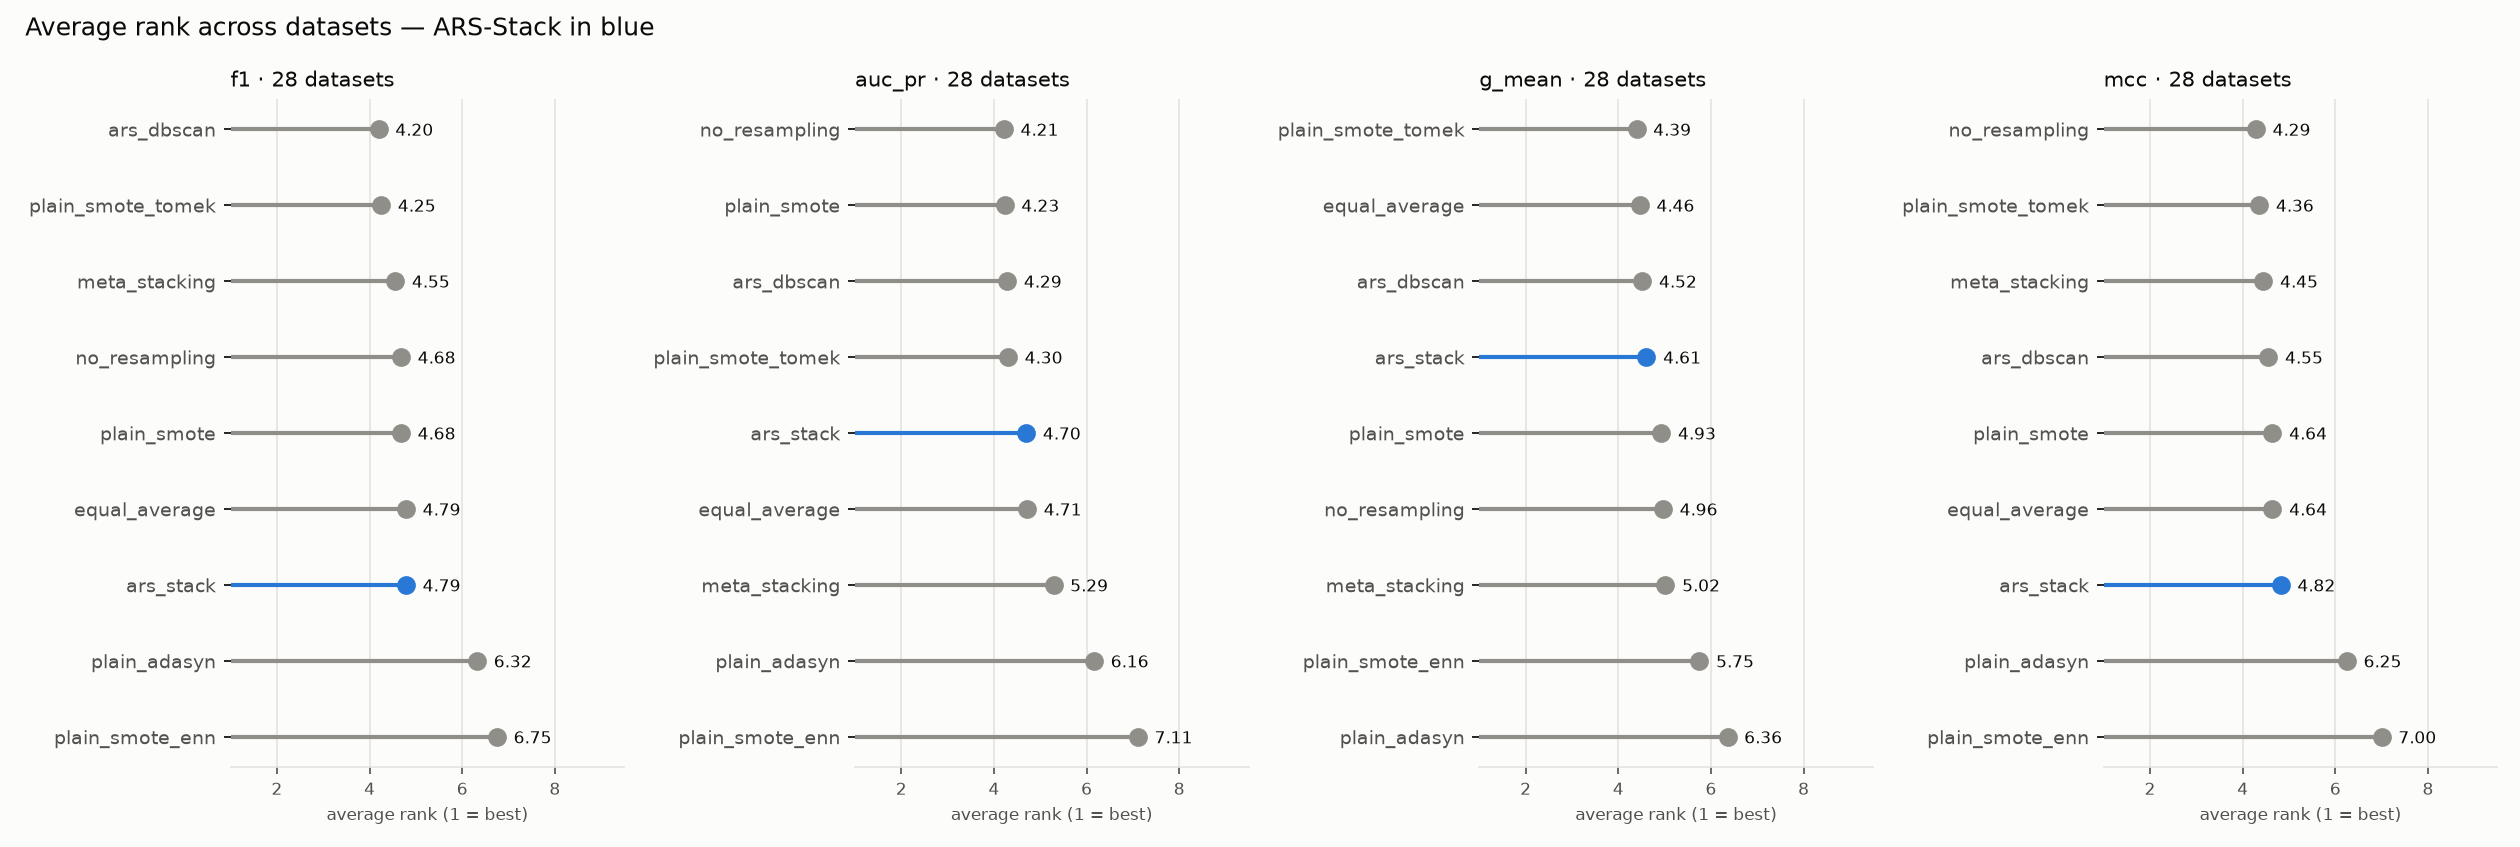
\includegraphics[width=\linewidth]{figures/average_ranks.png}
  \caption{Average rank per metric over 28 datasets (1 = best; \ars{} highlighted). Apart from SMOTE-ENN and ADASYN,
  all variants lie within about one rank of each other.}
  \label{fig:ranks}
\end{widefigure}

\para{Critical differences}
With 9 methods and 28 datasets, the Nemenyi critical difference is 2.27 ranks (Figure~\ref{fig:cd}). For AUC-PR,
SMOTE-ENN is significantly worse than every method ranked 4.84 or better, including \ars{}. For F1, it is
significantly worse only than ARS with DBSCAN (4.20) and SMOTE-Tomek (4.25), and \ars{} (4.79) is not separated from
it. No other pair of methods differs significantly.

\begin{widefigure}
  \centering
  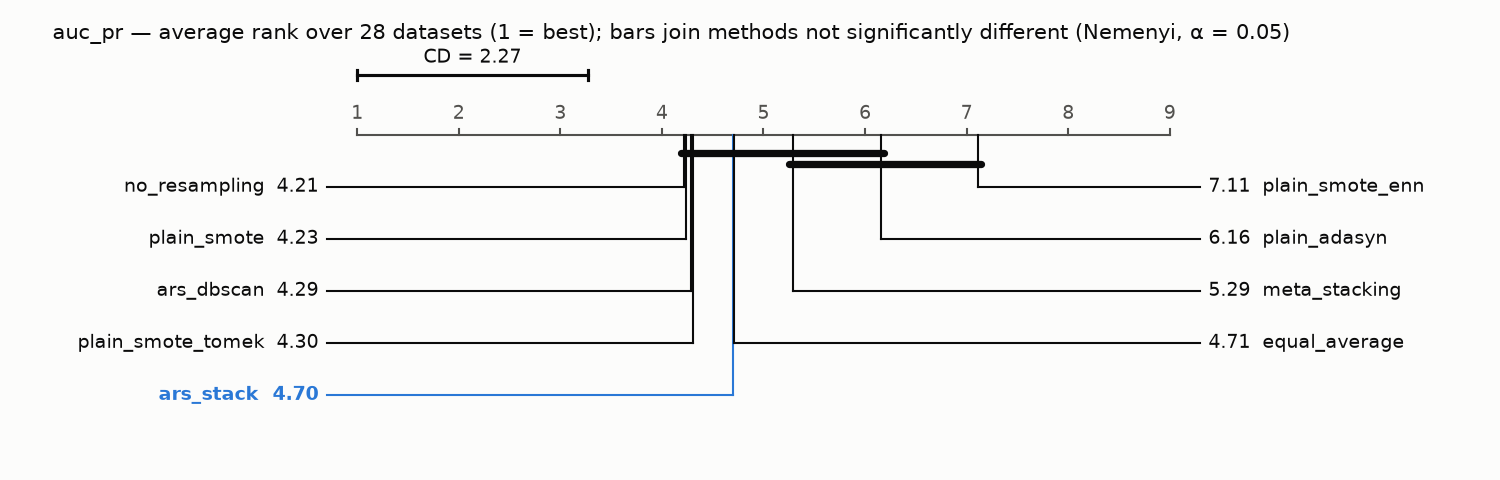
\includegraphics[width=0.49\linewidth]{figures/cd_auc_pr.png}\hfill
  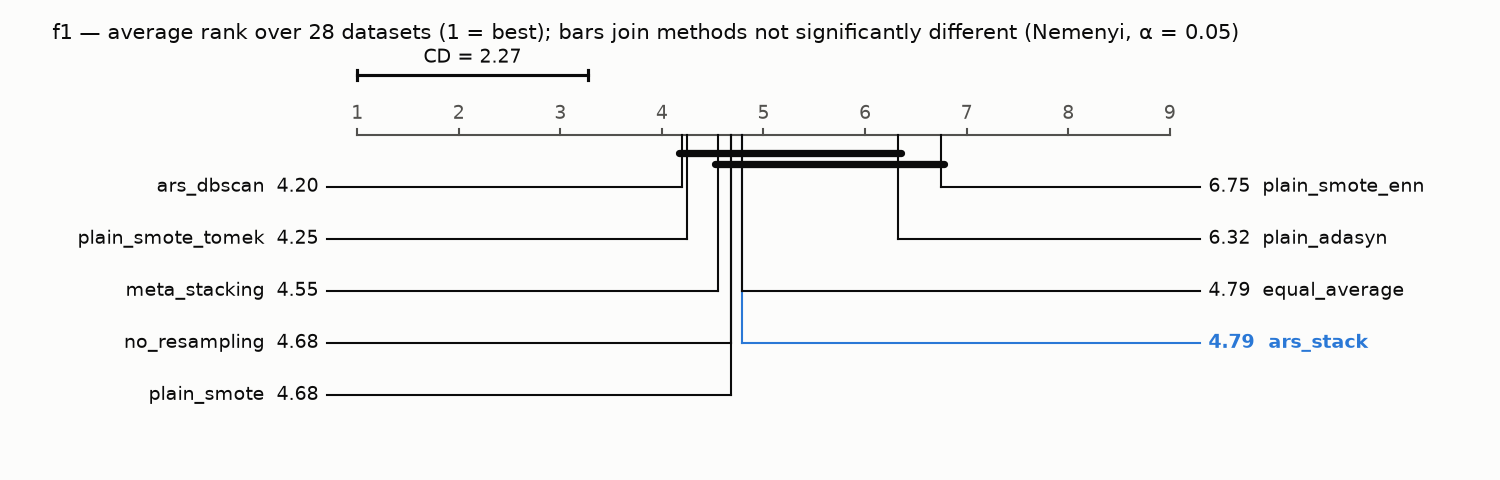
\includegraphics[width=0.49\linewidth]{figures/cd_f1.png}
  \caption{Critical-difference diagrams for AUC-PR (left) and F1 (right). Methods joined by a bar are not
  significantly different (Nemenyi, $\alpha=0.05$, CD $=2.27$).}
  \label{fig:cd}
\end{widefigure}

\para{Pairwise comparisons}
Holm-corrected Wilcoxon tests on per-dataset means (Table~\ref{tab:cross}) show \ars{} significantly better than
SMOTE-ENN on F1 (21 wins/7 losses, $p_{\mathrm{Holm}}=0.041$), AUC-PR (22/6, $p=0.049$) and MCC (22/6, $p=0.041$). Its
edge over ADASYN (19/9) does not survive correction ($p=0.089$ on F1). Against all other variants the win/loss counts
are near even, and the mean AUC-PR differences are small: $-0.0045$ against SMOTE, $-0.0062$ against No resampling,
and $+0.0001$ against equal weighting.

\begin{widetable}
  \centering
  \caption{\ars{} against each variant over 28 datasets: wins/ties/losses of \ars{}, mean difference $\Delta$
  (\ars{} $-$ baseline) and Holm-corrected Wilcoxon $p$ (bold: $p<0.05$).}
  \label{tab:cross}
  \footnotesize
  \setlength{\tabcolsep}{3.5pt}
  \begin{tabular}{lrrrrrrrrr}
\toprule
 & \multicolumn{3}{c}{F1} & \multicolumn{3}{c}{AUC-PR} & \multicolumn{3}{c}{MCC} \\
\cmidrule(lr){2-4}\cmidrule(lr){5-7}\cmidrule(lr){8-10}
ARS-Stack vs. & W/T/L & $\Delta$ & $p_{\mathrm{Holm}}$ & W/T/L & $\Delta$ & $p_{\mathrm{Holm}}$ & W/T/L & $\Delta$ & $p_{\mathrm{Holm}}$ \\
\midrule
Equal-weight avg. & 11/8/9 & +0.0003 & 1 & 12/3/13 & +0.0001 & 1 & 9/8/11 & +0.0003 & 1 \\
Meta-learner stacking & 13/3/12 & +0.0011 & 1 & 16/1/11 & +0.0019 & 0.983 & 12/3/13 & +0.0005 & 1 \\
ARS (DBSCAN) & 10/5/13 & +0.0017 & 1 & 9/5/14 & -0.0011 & 1 & 12/5/11 & +0.0024 & 1 \\
SMOTE & 11/0/17 & +0.0011 & 1 & 12/0/16 & -0.0045 & 0.879 & 11/0/17 & +0.0025 & 1 \\
SMOTE-Tomek & 11/0/17 & +0.0003 & 1 & 14/0/14 & -0.0041 & 0.983 & 11/0/17 & +0.0012 & 1 \\
ADASYN & 19/0/9 & +0.0088 & 0.089 & 19/0/9 & +0.0014 & 0.983 & 19/0/9 & +0.0079 & 0.117 \\
SMOTE-ENN & 21/0/7 & +0.0216 & \textbf{0.041} & 22/0/6 & +0.0176 & \textbf{0.048} & 22/0/6 & +0.0222 & \textbf{0.041} \\
No resampling & 14/0/14 & +0.0066 & 1 & 12/0/16 & -0.0062 & 1 & 13/0/15 & +0.0025 & 1 \\
\bottomrule
\end{tabular}

\end{widetable}

\para{Bayesian analysis}
The Bayesian signed-rank test (Table~\ref{tab:bayes}) can support equivalence. It shows:
\begin{itemize}
  \item \textbf{Practically better:} \ars{} beats SMOTE-ENN on F1 ($P=0.96$), AUC-PR ($0.98$) and MCC ($0.99$).
  \item \textbf{Practically equivalent} ($P(=)\geq0.95$) to SMOTE, SMOTE-Tomek, ARS with DBSCAN, equal-weight
        averaging and meta-learner stacking on all three metrics, and to ADASYN on AUC-PR and MCC.
  \item \textbf{Undecided} against No resampling. Equivalence is the most probable outcome ($P(=)=0.79$--$0.85$), and on
        AUC-PR No resampling is more likely better than worse (0.15 versus 0.003).
\end{itemize}
The per-dataset Bayesian correlated $t$-tests are mostly undecided with 15 folds. Where they decide, they confirm the
same picture: 76 of 112 dataset--metric pairs are equivalent to equal-weight averaging, and all 12 decided pairs against
SMOTE-ENN favour \ars{}.

\begin{widetable}
  \centering
  \caption{Bayesian signed-rank test over 28 datasets (ROPE $\pm0.01$): posterior probability that the baseline is
  practically better / equivalent / worse than \ars{}; a verdict needs $P\geq0.95$.}
  \label{tab:bayes}
  \footnotesize
  \setlength{\tabcolsep}{2.5pt}
  \begin{tabular}{lclclcl}
\toprule
 & \multicolumn{2}{c}{F1} & \multicolumn{2}{c}{AUC-PR} & \multicolumn{2}{c}{MCC} \\
\cmidrule(lr){2-3}\cmidrule(lr){4-5}\cmidrule(lr){6-7}
ARS-Stack vs. & $P(<)/P(=)/P(>)$ & Verdict & $P(<)/P(=)/P(>)$ & Verdict & $P(<)/P(=)/P(>)$ & Verdict \\
\midrule
Equal-weight avg. & 0.00/1.00/0.00 & equiv. & 0.00/1.00/0.00 & equiv. & 0.00/1.00/0.00 & equiv. \\
Meta-learner stacking & 0.00/1.00/0.00 & equiv. & 0.00/1.00/0.00 & equiv. & 0.00/1.00/0.00 & equiv. \\
ARS (DBSCAN) & 0.00/1.00/0.00 & equiv. & 0.00/1.00/0.00 & equiv. & 0.00/1.00/0.00 & equiv. \\
SMOTE & 0.00/1.00/0.00 & equiv. & 0.01/0.99/0.00 & equiv. & 0.00/0.99/0.01 & equiv. \\
SMOTE-Tomek & 0.00/1.00/0.00 & equiv. & 0.00/1.00/0.00 & equiv. & 0.00/0.99/0.00 & equiv. \\
ADASYN & 0.00/0.95/0.05 & undecided & 0.00/1.00/0.00 & equiv. & 0.00/0.98/0.02 & equiv. \\
SMOTE-ENN & 0.00/0.04/0.96 & ARS better & 0.00/0.02/0.98 & ARS better & 0.00/0.01/0.99 & ARS better \\
No resampling & 0.03/0.79/0.18 & undecided & 0.15/0.85/0.00 & undecided & 0.10/0.82/0.08 & undecided \\
\bottomrule
\end{tabular}

\end{widetable}

\para{Per-dataset results}
Table~\ref{tab:perds} lists every dataset with its characteristics and mean AUC-PR, ordered by minority-class size.
No resampling has the highest AUC-PR on 12 of the 28 datasets. On webpage, us\_crime, scene and wine\_quality, every
resampling variant loses 0.03--0.09 AUC-PR against it. Resampling wins mostly on datasets with tiny minority classes
(arrhythmia, oil, ozone\_level, abalone\_19). Saturated datasets (pen\_digits, car\_eval\_4, letter\_img,
optical\_digits) leave all variants within 0.002 of each other, except SMOTE-ENN on car\_eval\_4.

For the core datasets (Table~\ref{tab:core}), the variants on creditcard differ by less than a standard deviation, and
No resampling is best on mammography for every metric except G-mean. On 10-class yeast, resampling gives the largest
gains in the study: macro-F1 rises from 0.441 to 0.524 and G-mean from 0.642 to 0.708. SMOTE-ENN, by contrast,
collapses MCC to 0.388.

\begin{widetable}
  \centering
  \caption{Datasets and mean AUC-PR over 15 folds (best per dataset in bold), ordered by minority-class size. $n$:
  samples after duplicate removal; $d$: features; Min.: minority (smallest-class) size; IR: imbalance ratio.
  Core datasets are marked $^\ast$.}
  \label{tab:perds}
  \scriptsize
  \setlength{\tabcolsep}{3pt}
  \begin{tabular}{lrrrrrrrrrrr}
\toprule
 & & & & & \multicolumn{7}{c}{Mean AUC-PR} \\
\cmidrule(l){6-12}
Dataset & $n$ & $d$ & Min. & IR & None & SMOTE & SM-Tomek & ADASYN & SM-ENN & Meta & ARS \\
\midrule
yeast (10-class)$^\ast$ & 1,453 & 8 & 5 & 87.6 & 0.591 & \textbf{0.599} & 0.599 & 0.586 & 0.566 & 0.579 & 0.597 \\
libras\_move & 330 & 90 & 24 & 12.8 & 0.881 & 0.895 & 0.895 & 0.881 & 0.878 & \textbf{0.899} & 0.894 \\
arrhythmia & 452 & 278 & 25 & 17.1 & 0.815 & 0.833 & 0.833 & 0.837 & 0.783 & 0.840 & \textbf{0.843} \\
abalone\_19 & 4,177 & 10 & 32 & 129.5 & 0.049 & 0.068 & \textbf{0.075} & 0.056 & 0.056 & 0.058 & 0.055 \\
ecoli & 336 & 7 & 35 & 8.6 & 0.702 & 0.714 & 0.682 & \textbf{0.719} & 0.651 & 0.686 & 0.682 \\
oil & 937 & 49 & 41 & 21.9 & 0.580 & \textbf{0.622} & \textbf{0.622} & 0.620 & 0.573 & 0.603 & 0.600 \\
spectrometer & 531 & 93 & 45 & 10.8 & \textbf{0.913} & 0.878 & 0.885 & 0.854 & 0.858 & 0.865 & 0.865 \\
solar\_flare\_m0 & 412 & 32 & 58 & 6.1 & 0.186 & 0.177 & 0.178 & 0.175 & \textbf{0.246} & 0.192 & 0.193 \\
car\_eval\_4 & 1,728 & 21 & 65 & 25.6 & 0.999 & 1.000 & 1.000 & 1.000 & 0.972 & \textbf{1.000} & \textbf{1.000} \\
ozone\_level & 2,536 & 72 & 73 & 33.7 & 0.321 & 0.369 & 0.369 & 0.361 & \textbf{0.385} & 0.355 & 0.356 \\
car\_eval\_34 & 1,728 & 21 & 134 & 11.9 & 0.990 & 0.989 & 0.989 & 0.990 & 0.973 & \textbf{0.990} & 0.990 \\
us\_crime & 1,994 & 100 & 150 & 12.3 & \textbf{0.594} & 0.546 & 0.548 & 0.546 & 0.523 & 0.549 & 0.550 \\
scene & 2,400 & 294 & 173 & 12.9 & \textbf{0.271} & 0.242 & 0.245 & 0.239 & 0.210 & 0.223 & 0.226 \\
wine\_quality & 3,961 & 11 & 173 & 21.9 & \textbf{0.322} & 0.282 & 0.280 & 0.274 & 0.271 & 0.251 & 0.249 \\
yeast\_ml8 & 2,417 & 103 & 178 & 12.6 & \textbf{0.108} & 0.104 & 0.104 & 0.103 & 0.105 & 0.108 & 0.107 \\
thyroid\_sick & 3,771 & 52 & 231 & 15.3 & \textbf{0.954} & 0.946 & 0.947 & 0.947 & 0.893 & 0.944 & 0.946 \\
mammography$^\ast$ & 7,849 & 6 & 254 & 29.9 & \textbf{0.780} & 0.766 & 0.767 & 0.739 & 0.722 & 0.760 & 0.763 \\
sick\_euthyroid & 3,109 & 42 & 285 & 9.9 & \textbf{0.898} & 0.897 & 0.897 & 0.896 & 0.868 & 0.897 & 0.896 \\
abalone & 4,177 & 10 & 391 & 9.7 & 0.297 & 0.302 & 0.305 & 0.298 & \textbf{0.317} & 0.291 & 0.290 \\
creditcard$^\ast$ & 283,726 & 30 & 473 & 598.8 & 0.840 & \textbf{0.844} & \textbf{0.844} & 0.836 & 0.830 & 0.843 & 0.843 \\
optical\_digits & 5,620 & 64 & 554 & 9.1 & \textbf{0.995} & 0.995 & 0.995 & 0.994 & 0.994 & 0.995 & 0.995 \\
coil\_2000 & 8,380 & 85 & 568 & 13.8 & 0.126 & 0.125 & 0.124 & 0.124 & \textbf{0.140} & 0.119 & 0.124 \\
isolet & 7,797 & 617 & 600 & 12.0 & \textbf{0.967} & 0.962 & 0.962 & 0.960 & 0.867 & 0.959 & 0.962 \\
satimage & 6,435 & 36 & 626 & 9.3 & 0.809 & \textbf{0.811} & 0.811 & 0.805 & 0.728 & 0.806 & 0.811 \\
letter\_img & 18,668 & 16 & 640 & 28.2 & \textbf{0.996} & 0.995 & 0.995 & 0.995 & 0.995 & 0.995 & 0.995 \\
webpage & 34,780 & 300 & 981 & 34.5 & \textbf{0.855} & 0.814 & 0.814 & 0.788 & 0.761 & 0.788 & 0.814 \\
pen\_digits & 10,992 & 16 & 1,055 & 9.4 & 0.998 & 0.998 & 0.998 & 0.997 & 0.998 & \textbf{0.999} & \textbf{0.999} \\
protein\_homo & 144,968 & 74 & 1,251 & 114.9 & 0.885 & 0.901 & 0.901 & 0.888 & 0.893 & 0.901 & \textbf{0.902} \\
\midrule
Mean & & & & & 0.669 & 0.667 & 0.667 & 0.661 & 0.645 & 0.660 & 0.662 \\
\bottomrule
\end{tabular}

\end{widetable}

\begin{table}
  \centering
  \caption{Core datasets: mean $\pm$ standard deviation over 15 folds (best in bold).}
  \label{tab:core}
  \scriptsize
  \setlength{\tabcolsep}{2pt}
  \resizebox{\linewidth}{!}{\begin{tabular}{lrrrr}
\toprule
Variant & F1 & AUC-PR & G-mean & MCC \\
\midrule
\multicolumn{5}{l}{\textit{creditcard}} \\
\quad No resampling & \textbf{0.852 $\pm$ 0.023} & 0.840 $\pm$ 0.027 & 0.889 $\pm$ 0.019 & \textbf{0.855 $\pm$ 0.023} \\
\quad SMOTE & 0.846 $\pm$ 0.026 & 0.844 $\pm$ 0.028 & \textbf{0.890 $\pm$ 0.018} & 0.848 $\pm$ 0.026 \\
\quad SMOTE-ENN & 0.829 $\pm$ 0.031 & 0.830 $\pm$ 0.032 & 0.888 $\pm$ 0.024 & 0.830 $\pm$ 0.031 \\
\quad Meta-learner stacking & 0.846 $\pm$ 0.022 & 0.843 $\pm$ 0.026 & 0.885 $\pm$ 0.016 & 0.849 $\pm$ 0.022 \\
\quad ARS-Stack & 0.846 $\pm$ 0.022 & 0.843 $\pm$ 0.027 & 0.886 $\pm$ 0.015 & 0.848 $\pm$ 0.022 \\
\multicolumn{5}{l}{\textit{mammography}} \\
\quad No resampling & \textbf{0.709 $\pm$ 0.049} & \textbf{0.780 $\pm$ 0.042} & 0.824 $\pm$ 0.044 & \textbf{0.703 $\pm$ 0.050} \\
\quad SMOTE & 0.699 $\pm$ 0.041 & 0.766 $\pm$ 0.047 & 0.815 $\pm$ 0.038 & 0.693 $\pm$ 0.041 \\
\quad SMOTE-ENN & 0.662 $\pm$ 0.040 & 0.722 $\pm$ 0.058 & \textbf{0.833 $\pm$ 0.043} & 0.654 $\pm$ 0.040 \\
\quad Meta-learner stacking & 0.699 $\pm$ 0.051 & 0.760 $\pm$ 0.046 & 0.813 $\pm$ 0.050 & 0.696 $\pm$ 0.049 \\
\quad ARS-Stack & 0.694 $\pm$ 0.052 & 0.763 $\pm$ 0.046 & 0.801 $\pm$ 0.048 & 0.693 $\pm$ 0.049 \\
\multicolumn{5}{l}{\textit{yeast (10-class)}} \\
\quad No resampling & 0.441 $\pm$ 0.043 & 0.591 $\pm$ 0.057 & 0.642 $\pm$ 0.029 & 0.444 $\pm$ 0.041 \\
\quad SMOTE & 0.520 $\pm$ 0.060 & 0.599 $\pm$ 0.038 & 0.701 $\pm$ 0.043 & 0.447 $\pm$ 0.034 \\
\quad SMOTE-ENN & 0.461 $\pm$ 0.045 & 0.566 $\pm$ 0.047 & \textbf{0.725 $\pm$ 0.043} & 0.388 $\pm$ 0.032 \\
\quad Meta-learner stacking & 0.527 $\pm$ 0.062 & 0.579 $\pm$ 0.062 & 0.710 $\pm$ 0.041 & \textbf{0.471 $\pm$ 0.025} \\
\quad ARS-Stack & 0.524 $\pm$ 0.064 & 0.597 $\pm$ 0.041 & 0.708 $\pm$ 0.045 & 0.447 $\pm$ 0.032 \\
\bottomrule
\end{tabular}
}
\end{table}

\iffullversion
\begin{figure}
  \centering
  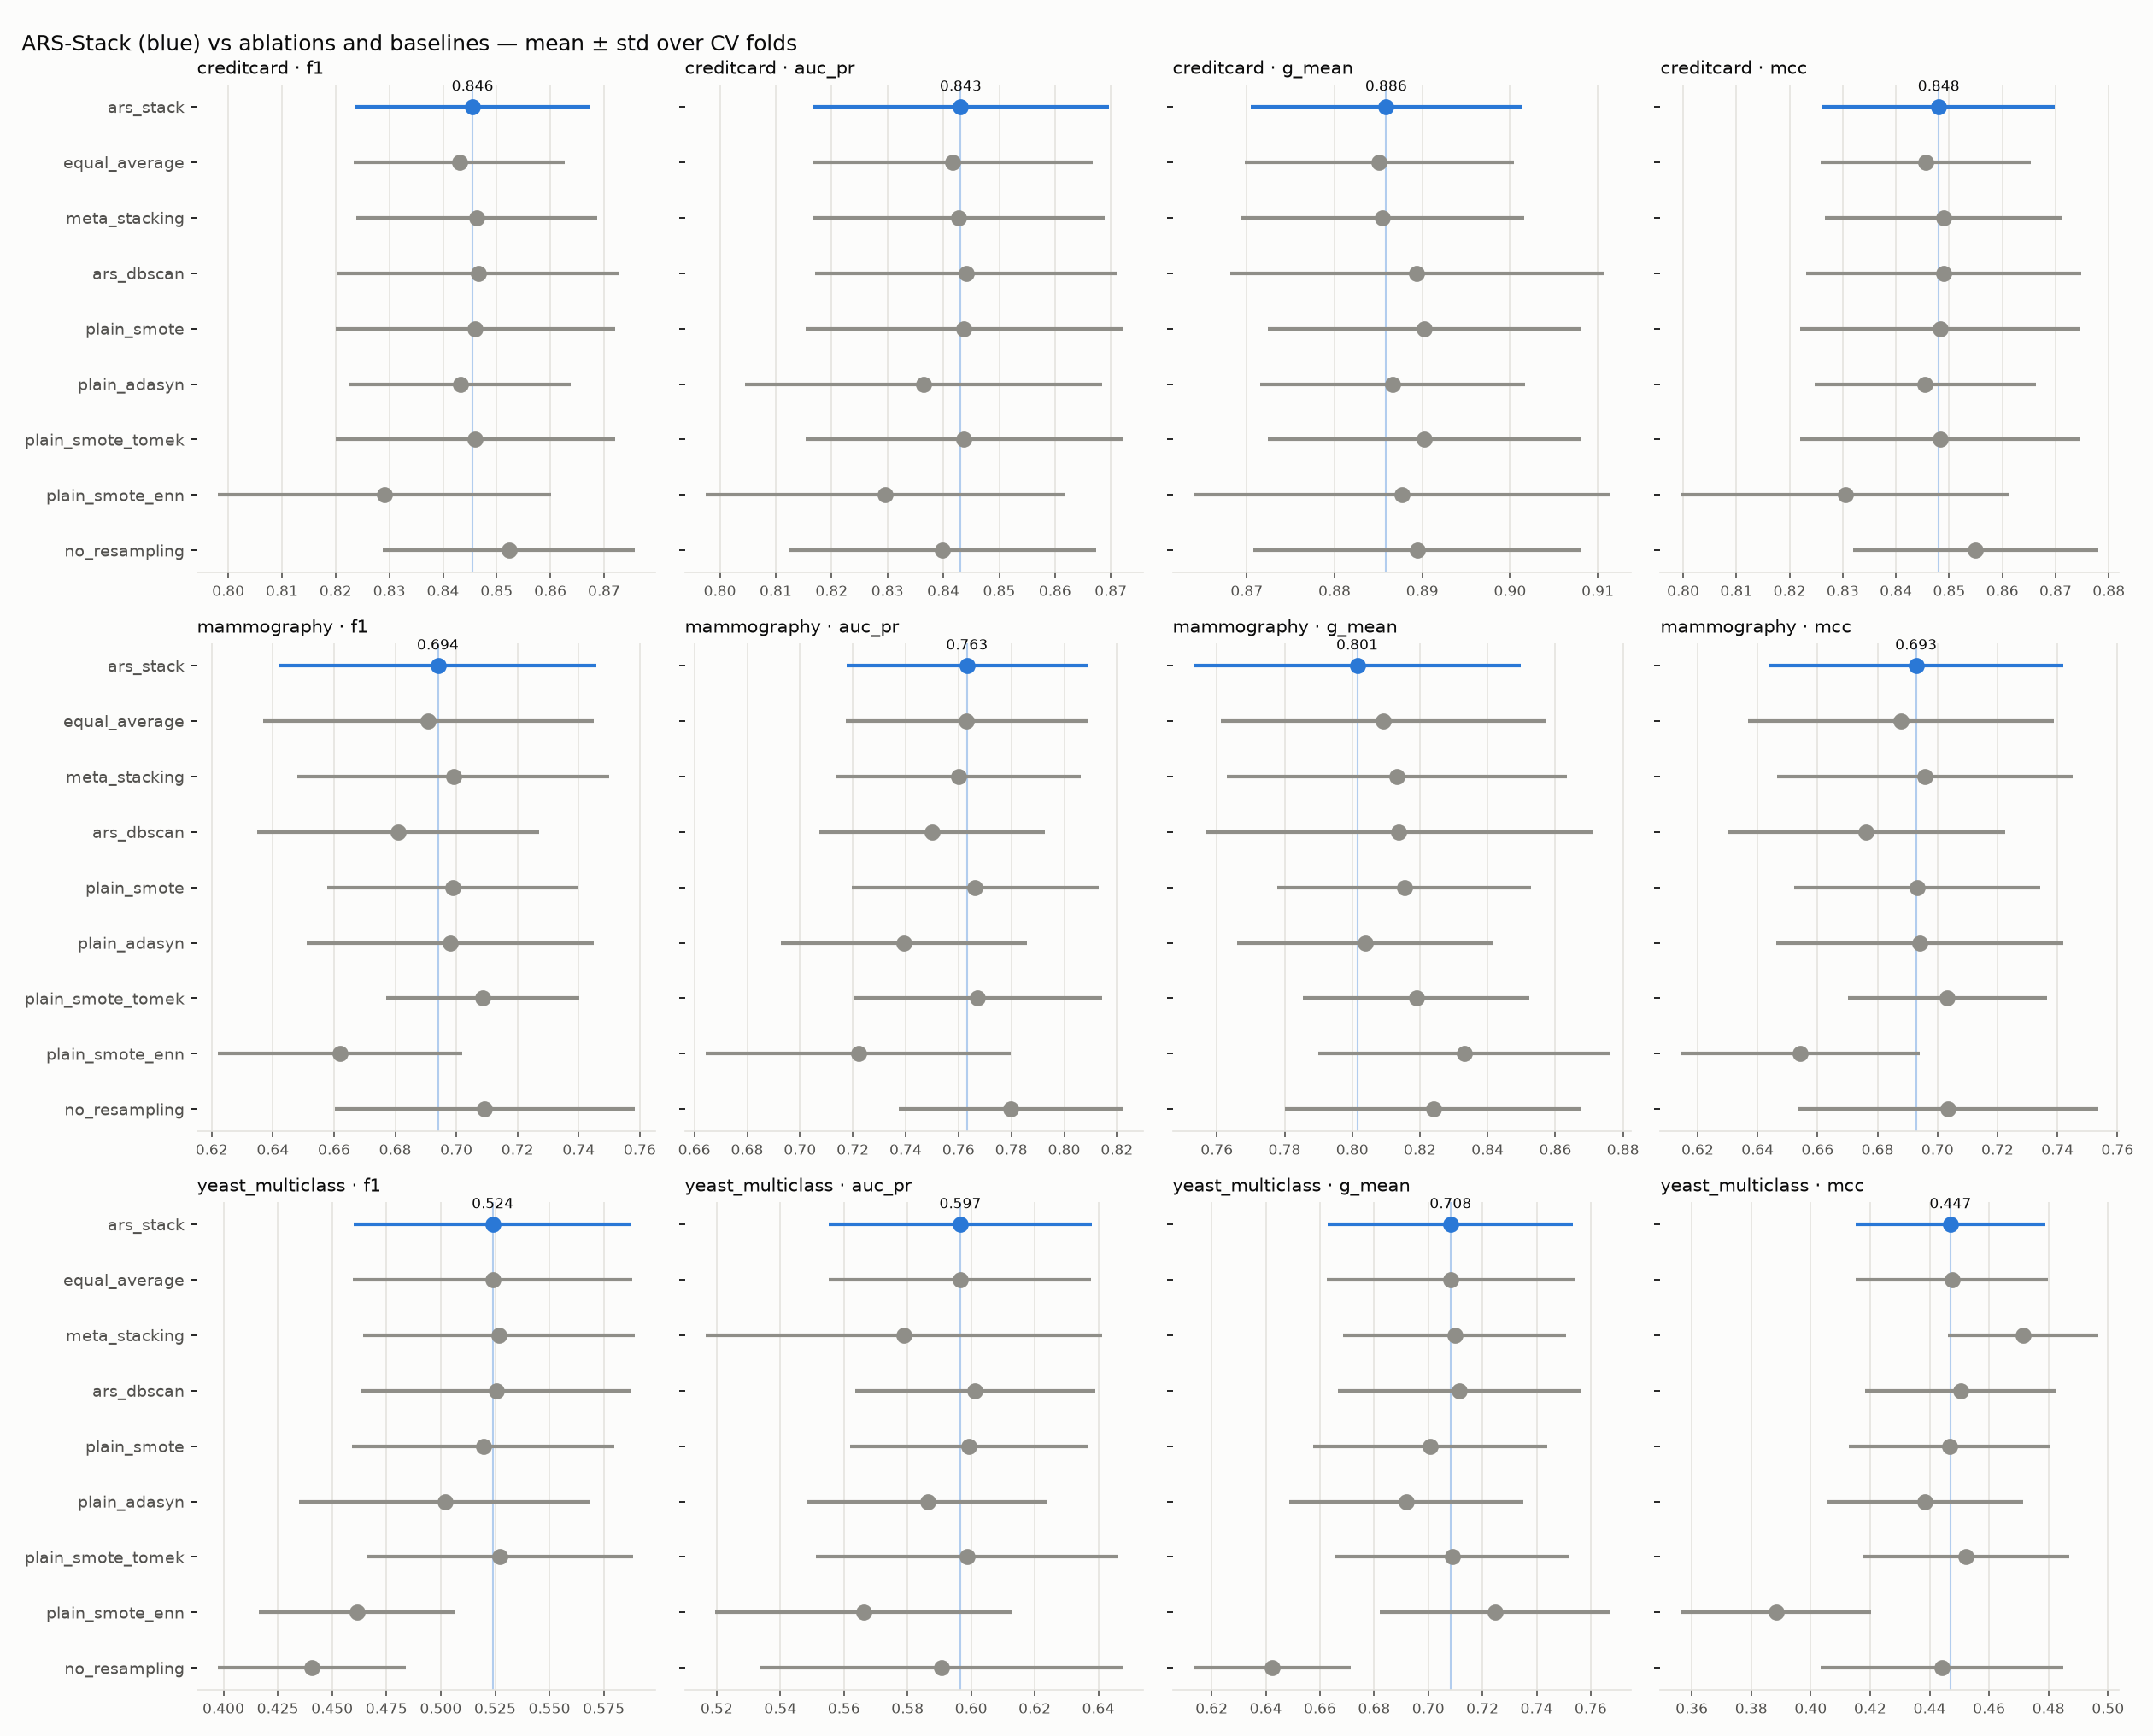
\includegraphics[width=0.78\linewidth]{figures/core_comparison.png}
  \caption{Core datasets: mean $\pm$ standard deviation over 15 folds for all nine variants and four metrics
  (\ars{} highlighted). Fold-to-fold spread exceeds most differences between variants.}
  \label{fig:core}
\end{figure}
\fi

\para{Literature baselines}
Reproducing the ``SMOTE + learner'' baselines of our review on a fixed split with a 0.5 threshold
(Table~\ref{tab:lit}) gives lower scores than published: creditcard F1 is 0.78--0.83 against the reported
0.89--0.915. Three leakage-free choices account for the gap: we remove duplicates, apply SMOTE only after splitting,
and hold the test set out. Oversampling before the split, common in applied work, lets synthetic interpolations of
test points leak into training. The comparison is indicative only, since the published splits differ.

\begin{table}
  \centering
  \caption{Literature baselines on a fixed split (0.5 threshold) versus reported values.}
  \label{tab:lit}
  \scriptsize
  \setlength{\tabcolsep}{2pt}
  \resizebox{\linewidth}{!}{\begin{tabular}{lllrrr}
\toprule
Dataset & Model & Source & F1 & AUC-PR & MCC \\
\midrule
creditcard & RandomForest + SMOTE & ours & 0.832 & 0.821 & 0.836 \\
creditcard & XGBoost + SMOTE & ours & 0.775 & 0.818 & 0.775 \\
creditcard & Simple Stacking (RF+XGB, LR meta) + SMOTE & ours & 0.815 & 0.823 & 0.815 \\
creditcard & Paper 7: xgboost & reported & 0.890 & 0.930 & -- \\
creditcard & Paper 7: easyensemble & reported & 0.870 & -- & -- \\
creditcard & Paper 9: stacking & reported & -- & -- & -- \\
creditcard & Paper 10: stacking smote tomek & reported & 0.915 & 0.900 & -- \\
mammography & RandomForest + SMOTE & ours & 0.615 & 0.606 & 0.602 \\
mammography & XGBoost + SMOTE & ours & 0.630 & 0.639 & 0.618 \\
mammography & Simple Stacking (RF+XGB, LR meta) + SMOTE & ours & 0.647 & 0.636 & 0.635 \\
\bottomrule
\end{tabular}
}
\end{table}
